\chapter{\label{cha:sts_state_of_the_art_methods}Vector Aggregation based STS Methods}

One of the key factors that contributed to the success of neural architectures in NLP is the fact that they are trained on large datasets. The biggest challenge that neural-based architectures face when applied to STS tasks is the small size of the datasets available to train them. As a result, in many cases, the networks cannot be trained properly. Given the huge amount of human labour required to produce STS datasets, it is not feasible to have high-quality large training datasets. As a result, researchers working in the field have considered unsupervised methods for STS. Recent unsupervised approaches use pre-trained word/sentence embeddings directly for the similarity task, without training a neural network model on them. Such approaches have used cosine similarity on sent2vec \autocite{pagliardini-etal-2018-unsupervised}, InferSent \autocite{conneau-EtAl:2017:EMNLP2017}, Word Mover's Distance \autocite{pmlr-v32-le14}, Doc2Vec \autocite{pmlr-v32-le14} and Smooth Inverse Frequency with GloVe vectors \autocite{DBLP:conf/iclr/AroraLM17}. While these approaches have produced decent results in the final rankings of shared tasks, they also act as strong baselines for the STS task. 

This chapter explores the performance of three unsupervised STS methods - cosine similarity using average vectors \autocite{mitchell-lapata-2008-vector}, Word Mover's Distance \autocite{10.5555/3045118.3045221} and cosine similarity using Smooth Inverse Frequency \autocite{DBLP:conf/iclr/AroraLM17}, and how to improve these methods using contextual word embeddings which will be explained more in Section \ref{sec:state_related}. 

We address four research questions in this chapter:

\textbf{RQ1:} Can contextual word embedding models like BERT be used to improve unsupervised STS methods?

\textbf{RQ2:} How well such an unsupervised method performs compared to other popular supervised/ unsupervised STS methods?

\textbf{RQ3:} Can the proposed unsupervised STS method be easily adapted into different languages?

\textbf{RQ4:} How well the proposed unsupervised STS method performs in a different domain? 


The main contributions of this chapter are as follows.

\begin{enumerate}
	\item The Related Work Section (Section \ref{sec:state_related}) covers three unsupervised STS techniques to compute semantic similarity at sentence level. 
	
	\item We propose an improved unsupervised STS method based on contextual word embeddings and evaluate it on three English STS datasets, two non-English STS datasets and a bio-medical STS dataset which were introduced in Chapter \ref{cha:sts_introduction}.
	
	\item The code used for the experiments conducted is publicly available to the community\footnote{The public GitHub repository is available on \url{https://github.com/tharindudr/simple-sentence-similarity}}.
	
\end{enumerate}

The rest of this chapter is organised as follows. Section \ref{sec:state_related} describes the three unsupervised STS methods we experimented with in this section. Section \ref{sec:state_method} presents the methodology, the contextual word embeddings we used, followed by the results from comparing the English datasets with the baselines. Sections \ref{sec:state_languages} and \ref{sec:state_domains} show how our method can be applied to different languages and domains in addition to their results. The chapter finishes with conclusions and ideas for future research directions in unsupervised STS methods.


\section{Related Work}
\label{sec:state_related}
Given that a good STS metric is required for a variety of natural language processing fields, researchers have proposed a large number of such metrics. Before the shift of interest to neural networks, the majority of the proposed methods relied heavily on feature engineering. With the introduction of word embedding models, researchers focused more on neural representation for this task. 

As we mentioned before, there are two main approaches that employ neural representation models: unsupervised and supervised. Unsupervised methods use pre-trained word/sentence embeddings directly for the similarity task without training a neural network model on them. In contrast, supervised approaches use a machine learning model trained to predict the similarity using word embeddings \autocite{ranasinghe-etal-2019-enhancing}. Since this chapter focuses on unsupervised STS methods, this section contains previous research on unsupervised STS methods.


The three unsupervised STS methods explored in this chapter: Cosine similarity on average vectors \autocite{mitchell-lapata-2008-vector}, Word Mover's Distance \autocite{10.5555/3045118.3045221} and Cosine similarity using Smooth Inverse Frequency \autocite{DBLP:conf/iclr/AroraLM17}, are the most common unsupervised methods explored in STS tasks. Apart from these methods, cosine similarity of the output from Infersent \autocite{conneau-EtAl:2017:EMNLP2017}, sent2vec \autocite{pagliardini-etal-2018-unsupervised} and doc2vec \autocite{pmlr-v32-le14} have also been used to represent the similarity between two sentences which we discuss in the next chapter. 


\subsection{Cosine Similarity on Average Vectors}
The first unsupervised STS method that we considered to estimate the semantic similarity between a pair of sentences takes the average of the word embeddings of all words in the two sentences and calculates the cosine similarity between the resulting embeddings \autocite{mitchell-lapata-2008-vector}. This method is a common way to acquire sentence embeddings from word embeddings \autocite{orasan-2018-aggressive}. Obviously, this simple baseline leaves considerable room for variation. Researchers have investigated the effects of ignoring stopwords and computing an average weighted by tf-idf in particular \autocite{j.1551-6709.2010.01106.x}.

\subsection{Word Mover's Distance}
The second state-of-the-art STS method that we have considered is Word Mover's Distance introduced by \textcite{10.5555/3045118.3045221}. Word Mover's Distance uses the word embeddings of the words in two texts to measure the minimum distance that the words in one text need to ``travel'' in semantic space to reach the words in the other text as shown in Figure \ref{fig:WMD}. \cite{10.5555/3045118.3045221} shows that this is a better approach than vector averaging since this technique keeps the word vectors as it is, throughout the operation.

\begin{figure}[ht]
	\centering
	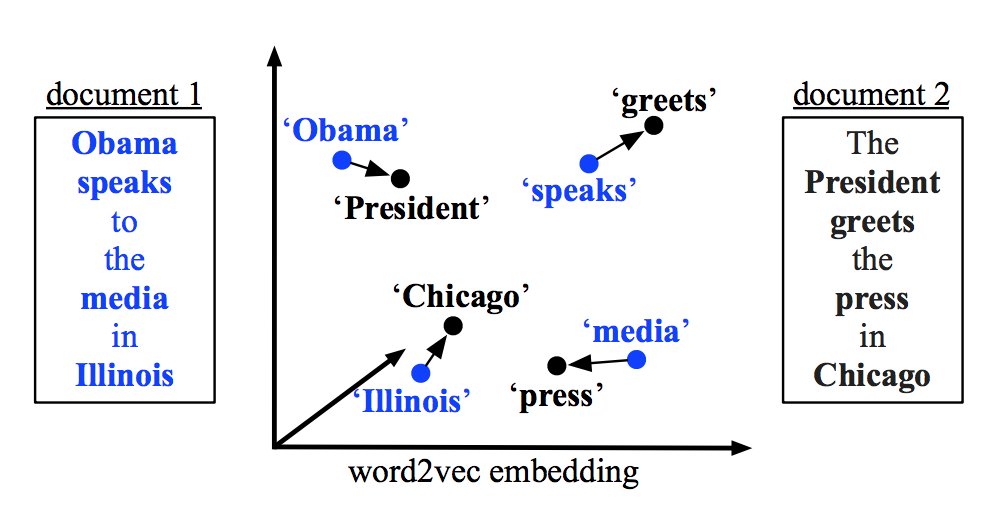
\includegraphics[scale=0.4]{figures/semantic_textual_similarity/state_of_the_art/word_movers_distance.png}
	\caption[The Word Mover's Distance between two sentences]{The Word Mover's Distance between two sentences \autocite{10.5555/3045118.3045221}}
	\label{fig:WMD}
\end{figure}

\subsection{Cosine Similarity Using Smooth Inverse Frequency}
The third and the last unsupervised STS method we considered is to acquire sentence embeddings using Smooth Inverse Frequency proposed by \cite{DBLP:conf/iclr/AroraLM17} and then calculate the cosine similarity between those sentence embeddings. Semantically speaking, taking the average of the word embeddings in a sentence tends to give too much weight to words that are fairly irrelevant. Smooth Inverse Frequency tries to solve this problem in two steps. 

\begin{enumerate}
	\item \textbf{Weighting}: Smooth Inverse Frequency takes the weighted average of the word embeddings in the sentence. Every word embedding is weighted by $a\over{a + p(w)}$, where $a$ is a parameter that is typically set to 0.001 and $p(w)$ is the estimated frequency of the word in a reference corpus. 
	\item \textbf{Common component removal}: After weighting, Smooth Inverse Frequency computes the principal component of the resulting embeddings for a set of sentences. It then subtracts their projections on the \textit{first principal component} from these sentence embeddings. This step should remove variations related to frequency and syntax that are less relevant semantically.
\end{enumerate}

As a result, Smooth Inverse Frequency downgrades non-content bearing words such as \emph{but, just}, etc., and keeps the information that contributes most to the semantics of the sentence \autocite{DBLP:conf/iclr/AroraLM17}. After acquiring the sentence embeddings for a pair of sentences, the cosine similarity between those two vectors was taken to represent their similarity. 

\noindent  All of these STS methods are based on word embeddings/vectors. The main weakness of word vectors is that each word has the same unique vector regardless of the context it appears. Consider the word "bank", which has several meanings. Still, in standard word embeddings such as GloVe \autocite{pennington-etal-2014-glove}, fastText \autocite{mikolov-etal-2018-advances} or Word2Vec  \autocite{10.5555/2999792.2999959} each instance of the word has the same representation regardless of the meaning which is used. For example, the word `bank' in two sentences - ``I am walking by the river bank'' and ``I deposited money to the bank'' would have the same embeddings, which can be confusing for machine learning models. The recent introduction of contextualised word representations such as BERT \autocite{devlin-etal-2019-bert} and XLNet \autocite{yang2019xlnet} solved this problem by providing vectors for words taking their context into consideration. In this way, the word 'bank' in the above sentences would have two different embeddings. Contextual word embedding models have improved the results of many natural language processing tasks over traditional word embedding models \autocite{peters-etal-2018-deep, devlin-etal-2019-bert}. However, they have not been applied to unsupervised vector aggregation-based STS methods to the best of our knowledge.


Therefore, we explore how contextualised word representations can improve the above mentioned unsupervised STS methods. We will explain the neural network architectures of these contextual word embeddings in Chapter \ref{cha:sts_transformers}. For this chapter, we considered these architectures as a black box where we feed the words to get the embeddings. We considered these contextualised word representations in terms of their popularity by the time we were doing the experiments.

\begin{enumerate}
\item \textbf{ELMo\footnote{More details about ELMo can be viewed on \url{https://allennlp.org/elmo}}}
introduced by \textcite{peters-etal-2018-deep}, uses bidirectional language model (biLM) to learn both the word (e.g., syntax and semantics) and linguistic context. After pre-training, an internal state of vectors can be transferred to downstream natural language processing tasks. ELMo vectors have been successfully used in many natural language processing tasks such as text classification \autocite{jiang-etal-2019-team} and named entity recognition \autocite{Luo2018}, which motivated us to explore ELMo in unsupervised STS methods. Also, we were aware of the fact that ELMo has been pre-trained on different languages \autocite{che-EtAl:2018:K18-2} and different domains \autocite{jin2019probing} which will be useful for when we are adapting our methodology for different languages and domains in Sections \ref{sec:state_languages} and \ref{sec:state_domains}.

\item \textbf{BERT\footnote{The GitHub repository of BERT is available on \url{https://github.com/google-research/bert}}} Introduced by \textcite{devlin-etal-2019-bert}, BERT is probably the most popular contextualised word embedding model. In contrast to ELMo which uses a shallow concatenation layer, BERT employs a deep concatenation layer. As a result, BERT is considered a very powerful embedding architecture. BERT has been successfully applied in many natural language processing tasks such as text classification \autocite{Ranasinghe2019a}, word similarity \autocite{hettiarachchi-etal-2020-brums}, named entity recognition \autocite{10.1145/3394486.3403149} and question and answering \autocite{yang-etal-2019-end}. Similarly to ELMo, BERT has been widely adapted for different languages\footnote{Information about pre-trained BERT models for different languages can be found on \url{https://bertlang.unibocconi.it/}} such as Arabic \autocite{antoun-etal-2020-arabert}, French \autocite{martin-etal-2020-camembert}, Spanish \autocite{CaneteCFP2020}, Greek \autocite{10.1145/3411408.3411440} etc. and different domains such as SciBERT \autocite{beltagy-etal-2019-scibert}, BioBERT \autocite{10.1093/bioinformatics/btz682}, LEGAL-BERT \autocite{chalkidis-etal-2020-legal} etc.  

\item \textbf{Flair\footnote{The GitHub repository of Flair is available on \url{https://github.com/flairNLP/flair}}} is another popular contextualised word embedding model introduced by \textcite{akbik-etal-2018-contextual}. It takes a different approach, using a character-level language model rather than the word level language model used in ELMo and BERT. Flair has also been used successfully in natural language processing tasks such as named entity recognition \autocite{akbik-etal-2019-pooled}, part-of-speech tagging \autocite{akbik-etal-2018-contextual} and has been widely adapted for different languages and domains \autocite{akbik-etal-2018-contextual,sharma2019bioflair}.

\end{enumerate}

Apart from using these contextual word embedding models individually, we also considered \textbf{Stacked Embeddings} of these models. Stacked Embeddings are obtained by concatenating different embeddings. According to \textcite{akbik-etal-2018-contextual}, stacking the embeddings can provide powerful embeddings to represent words. Therefore, we experimented with several combinations of Stacked Embeddings.

Even though these contextual word embedding models have shown promising results in many natural language processing tasks, to the best of our knowledge, none of these contextual word representations have been applied to unsupervised vector aggregation-based STS methods.  


\section{Improving State of the Art STS Methods}
\label{sec:state_method}
As mentioned before, we applied different contextual word embeddings on three unsupervised STS methods and their variants. First, we experimented with English STS datasets that we explained in Section \ref{sec:sts_intro_datsets}. Our implementation was based on the \textit{Flair-NLP} Framework \autocite{akbik-etal-2019-flair} which makes it easier to switch between different word embedding models when acquiring word embeddings. Additionally, \textit{Flair-NLP} has its own \textit{model zoo} of pre-trained models to allow researchers to use state-of-the-art NLP models in their applications. For English, all of these contextualised word embedding models come with different variants such as \textit{small, large etc}. Usually, the larger models provide a better accuracy since they have been trained on a larger dataset than the smaller models. However, this comes with the disadvantage that these larger models are more resource-intensive than the smaller models. To achieve better accuracy, we used the largest model available in each contextual word embedding model. We will describe these models in the following paragraphs. 

For ELMo, we used the `original (5.5B)' pre-trained model provided by \textcite{peters-etal-2018-deep} which was trained on a dataset of 5.5B tokens consisting of Wikipedia (1.9B) and all of the monolingual news crawl data from WMT\footnote{WMT: Workshop on Statistical Machine Translation is a leading conference in NLP that is being organised annually.} 2008-2012 (3.6B). \textcite{peters-etal-2018-deep} mention that ELMo original (5.5B) performs slightly better than other ELMo models and recommend it as the default model. Using this model, we represented each word as a vector with a size of 3072 dimensions.

For BERT, we used the `bert-large-cased' pre-trained model. Compared to the `bert-base-cased' model, this model provided slightly better results in all the NLP tasks experimented in \textcite{devlin-etal-2019-bert}. We represented each word as a 4096 lengthened vector using this model. 

As suggested in \textcite{akbik-etal-2018-contextual}, the recommended way to use Flair embeddings is to stack pre-trained `news-forward' flair embeddings and pre-trained flair `news-backward' embeddings with GloVe \autocite{pennington-etal-2014-glove} word embeddings. We used the stacked model to represent each word as a 4196 lengthened vector. 

As mentioned before, we also considered stacked embeddings of ELMo and BERT. For this, we used the pre-trained `bert-large-uncased' model and `original (5.5B)' pre-trained ELMo model to represent each word as a 4096 + 3072 vector.

To compare the results of the contextualised word embeddings, we used a standard word representation model as a baseline in each experiment. In this research, we used Word2vec embeddings \autocite{DBLP:journals/corr/abs-1301-3781} pre-trained on Google news corpus\footnote{Pretrained Word2vec can be downloaded from \url{https://code.google.com/archive/p/word2vec/}}. We represented each word as a 300 lengthened vector using this model.

In the following list, we show the performance of each unsupervised STS method with contextual word embeddings on the different English STS datasets. 

\begin{enumerate}
	\item \textbf{Cosine Similarity on Average Vectors} - The first unsupervised STS method we tried to improve using contextual word embeddings is Cosine Similarity on Average Vectors, as explained in Section \ref{sec:state_related}. Table \ref{tab:sick_average_vectors} shows the results for the SICK dataset, Table \ref{tab:sts_average_vectors} shows the results for the STS 2017 dataset and Table \ref{tab:quora_average_vectors} shows the results for the Quora Question Pairs dataset. To compare our results with other systems, we conducted the experiments only on the test data of the three above mentioned datasets. Since this method leaves considerable room for variation, we have investigated the following variations and reported their results in each table. 
	
	\begin{enumerate}
		\item All the word vectors were considered for averaging. Results are shown in column I of Tables \ref{tab:sick_average_vectors}, \ref{tab:sts_average_vectors} and \ref{tab:quora_average_vectors}
		
		\item All the word vectors except the vectors for stop words were considered for averaging. Column II of Tables \ref{tab:sick_average_vectors}, \ref{tab:sts_average_vectors} and \ref{tab:quora_average_vectors} shows the results. 
		
		\item All the word vectors were weighted from their tf-idf scores and considered averaging. Results are shown in column III of Tables \ref{tab:sick_average_vectors}, \ref{tab:sts_average_vectors} and \ref{tab:quora_average_vectors}
		
		\item Stop words were removed first and the remaining word vectors were weighted from their tf-idf scores and considered averaging. Column IV of Tables \ref{tab:sick_average_vectors}, \ref{tab:sts_average_vectors} and \ref{tab:quora_average_vectors} shows the results.  
		
	\end{enumerate}
	
\begin{table*}[htb]
	%\footnotesize
	\centering
	\scalebox{0.95}{
		\begin{tabular}{|l|cc|cc|cc|cc|}
			
			\hline & 
			\multicolumn{2}{c|}{\textbf{I}}    & \multicolumn{2}{c|}{\textbf{II}}   & \multicolumn{2}{c|}{\textbf{III}}  &    
			\multicolumn{2}{c|}{\textbf{IV}}   \\ 
			\hline
			\multicolumn{1}{|l|}{\textbf{Model}} 
			& $\bm{\rho}$   & $\bm{\tau}$     
			& $\bm{\rho}$   & $\bm{\tau}$  
			& $\bm{\rho}$   & $\bm{\tau}$  
			& $\bm{\rho}$   & $\bm{\tau}$  
			\\ \hline
			\textit{Word2vec}                  
			& \textbf{0.730}$^{\dagger}$  & 0.624        
			& \textbf{0.714}        & 0.583    
			& \textbf{0.693}        & 0.570    
			& \textbf{0.687}        & 0.555    \\
			\textit{ELMo}                     
			& 0.669                 & 0.592         
			& 0.693                 & 0.603       
			& 0.676                 & \textbf{0.579}  
			& 0.668                 & \textbf{0.572}      \\
			\textit{Flair}                     
			& 0.646                 & 0.568         
			& 0.670                 & 0.562       
			& 0.644                 & 0.535  
			& 0.643                 & 0.531      \\
			\textit{BERT}                     
			& 0.683                 & 0.633         
			& 0.686                 & 0.606       
			& 0.557                 & 0.552  
			& 0.539                 & 0.538 \\
			\textit{ELMo $\bigoplus$ BERT}                     
			& 0.696                 & \textbf{0.634}$^{\dagger}$          
			& 0.702                 & \textbf{0.614}       
			& 0.607                 & 0.562  
			& 0.591                 & 0.551 \\
			\hline
		\end{tabular}
	}
	\caption[Results for SICK with Vector Averaging]{Results for SICK dataset with Vector Averaging. Columns \textbf{I}, \textbf{II}, \textbf{III} and \textbf{IV} indicate the different variations as explained above. For each word embedding model, Pearson Correlation ($\bm{\rho}$) and Spearman Correlation ($\bm{\tau}$) are reported for all variations between the predicted values and the gold labels of the test set. $\bigoplus$ indicates a stacked word embedding model. The best result in each variation is highlighted in \textbf{Bold}. The best result from all of the variations is marked with ${\dagger}$. }  
	\label{tab:sick_average_vectors}
\end{table*}

\begin{table*}[htb]
	%\footnotesize
	\centering
	\scalebox{0.90}{
		\begin{tabular}{|l|cc|cc|cc|cc|}
			
			\hline & 
			\multicolumn{2}{c|}{\textbf{I}}    & \multicolumn{2}{c|}{\textbf{II}}   & \multicolumn{2}{c|}{\textbf{III}}  &    
			\multicolumn{2}{c|}{\textbf{IV}}   \\ 
			\hline
			\multicolumn{1}{|l|}{\textbf{Model}} 
			&  $\bm{\rho}$   & $\bm{\tau}$      
			&  $\bm{\rho}$   & $\bm{\tau}$  
			&  $\bm{\rho}$   & $\bm{\tau}$  
			&  $\bm{\rho}$   & $\bm{\tau}$  
			\\ \hline
			\textit{Word2vec}                     
			& \textbf{0.625} & 0.583         
			& 0.609             & \textbf{0.635}$^{\dagger}$       
			& \textbf{0.640}$^{\dagger}$    & \textbf{0.591} 
			& \textbf{0.588}    & \textbf{0.573} \\
			\textit{ELMo}                     
			& 0.575                      & 0.574         
			& \textbf{0.618}             & 0.609       
			& 0.374                      & 0.395  
			& 0.352                      & 0.376 \\
			\textit{Flair}                     
			& 0.411                      & 0.444         
			& 0.584                      & 0.586       
			& 0.325                      & 0.374  
			& 0.336                      & 0.386 \\
			\textit{BERT}                     
			& 0.575                      & 0.574         
			& 0.555                      & 0.588       
			& 0.355                      & 0.401  
			& 0.309                      & 0.386 \\
			\textit{ELMo $\bigoplus$ BERT}                     
			& 0.600                      & \textbf{0.597}       
			& 0.591                      & 0.608       
			& 0.391                      & 0.413  
			& 0.354                      & 0.398 \\
			\hline
		\end{tabular}
	}
	\caption[Results for STS 2017 with Vector Averaging]{Results for STS 2017 dataset with Vector Averaging. Columns \textbf{I}, \textbf{II}, \textbf{III} and \textbf{IV} indicate the different variations as explained above. For each word embedding model, Pearson Correlation ($\bm{\rho}$) and Spearman Correlation ($\bm{\tau}$) are reported for all variations between the predicted values and the gold labels of the test set. $\bigoplus$ indicates a stacked word embedding model. The best result in each variation is highlighted in \textbf{Bold}. The best result from all of the variations is marked with ${\dagger}$. }  
	\label{tab:sts_average_vectors}
\end{table*}

\begin{table*}[htb]
	%\footnotesize
	\centering
	\scalebox{0.90}{
		\begin{tabular}{|l|c|c|c|c|}
			
			\hline
			& \multicolumn{1}{c|}{\textbf{I}} & \multicolumn{1}{c|}{\textbf{II}}             & \multicolumn{1}{c|}{\textbf{III}}  &    
			\multicolumn{1}{c|}{\textbf{IV}} \\ 
			\hline
			\multicolumn{1}{|l|}{\textbf{Model}} & RMSE   & RMSE     &  RMSE & RMSE 
			\\ \hline
			\textit{Word2vec}  
			& \textbf{0.621}                      & \textbf{0.591}$^{\dagger}$    
			& \textbf{0.646}                      & \textbf{0.607}       \\
			\textit{ELMo}  
			& 0.629                      & 0.615    
			& 0.652                      & 0.649       \\
			\textit{Flair}  
			& 0.720                      & 0.711    
			& 0.743                      & 0.735       \\
			\textit{BERT}  
			& 0.651                      & 0.643    
			& 0.673                      & 0.662       \\
			\textit{ELMo $\bigoplus$ BERT}  
			& 0.625                      & 0.611    
			& 0.650                      & 0.647       \\	
			\hline
		\end{tabular}
	}
	\caption[Results for QUORA with Vector Averaging]{Results for QUORA dataset with Vector Averaging. Columns \textbf{I}, \textbf{II}, \textbf{III} and \textbf{IV} indicate the different variations as explained above. For each word embedding model, Root Mean Squared Error (RMSE) is reported for all variations. $\bigoplus$ indicates a stacked word embedding model. The best result in each variation is highlighted in \textbf{Bold}. The best result from all of the variations is marked with ${\dagger}$. }  
	\label{tab:quora_average_vectors}
\end{table*}

	From the results in Tables \ref{tab:sick_average_vectors}, \ref{tab:sts_average_vectors} and \ref{tab:quora_average_vectors} there is no clear indication that contextualised word embeddings perform better than the standard word embeddings. In all of the datasets considered, the best result was provided by Word2vec. 
	
	All the contextualised word embedding models we considered have more than 3000 dimensions for the word representation, which is higher than the number of dimensions for the word representation we had for standard embeddings - 300. As the vector averaging model is highly dependent on the number of dimensions that a vector can have, the curse of dimensionality might be the reason for the poor performance of contextualised word embeddings in vector averaging variants \autocite{ranasinghe-etal-2019-enhancing}.

	
	\item \textbf{Word Mover's Distance} - The second unsupervised STS method we experimented with is Word Mover's Distance, as explained in Section \ref{sec:state_related}. Similarly to the average vectors, we compared having contextualised word embeddings in place of traditional word embeddings in Word Mover's Distance. Table \ref{tab:sick_word_movers} shows the results for the SICK dataset. Table \ref{tab:sts_word_movers} shows the results for the STS 2017 dataset and Table \ref{tab:quora_word_movers} shows the results for the Quora Questions Pairs dataset. We have investigated the effects of considering/ ignoring stop words before calculating the Word Mover's Distance as detailed below. 
	
	\begin{enumerate}
		\item Considering all the words to calculate the Word Mover's Distance. Results are shown in column I of Tables \ref{tab:sick_word_movers}, \ref{tab:sts_word_movers} and \ref{tab:quora_word_movers}
		\item Removing stop words before calculating the Word Mover's Distance. Column II of Tables \ref{tab:sick_word_movers}, \ref{tab:sts_word_movers} and \ref{tab:quora_word_movers} shows the results. 
	\end{enumerate} 
	
	

\begin{table*}[htb]
	%\footnotesize
	\centering
	\scalebox{0.95}{
		\begin{tabular}{|l|cc|cc|}
			
			\hline & 
			\multicolumn{2}{c|}{\textbf{I}}    & \multicolumn{2}{c|}{\textbf{II}}   \\ 
			\hline
			\multicolumn{1}{|l|}{\textbf{Model}} 
			& $\bm{\rho}$   & $\bm{\tau}$     
			& $\bm{\rho}$   & $\bm{\tau}$  
			\\ \hline
			\textit{Word2vec}                  
			& \textbf{0.730}$^{\dagger}$  & 0.624        
			& \textbf{0.714}        & 0.583   \\
			\textit{ELMo}                     
			& 0.669                 & 0.592         
			& 0.693                 & 0.603    \\
			\textit{Flair}                     
			& 0.646                 & 0.568         
			& 0.670                 & 0.562    \\
			\textit{BERT}                     
			& 0.683                 & 0.633         
			& 0.686                 & 0.606  \\
			\textit{ELMo $\bigoplus$ BERT}                     
			& 0.696                 & \textbf{0.634}$^{\dagger}$          
			& 0.702                 & \textbf{0.614}  \\
			\hline
		\end{tabular}
	}
	\caption[Results for SICK with Word Mover's Distance]{Results for SICK dataset with Word Mover's Distance. Columns \textbf{I} and \textbf{II} indicate the different variations as explained above. For each word embedding model, Pearson Correlation ($\bm{\rho}$) and Spearman Correlation ($\bm{\tau}$) are reported on all variations between the predicted values and the gold labels of the test set. $\bigoplus$ indicates a stacked word embedding model. The best result in each variation is highlighted in \textbf{Bold}. The best result from all of the variations is marked with ${\dagger}$. }  
	\label{tab:sick_word_movers}
\end{table*}

\begin{table*}[htb]
	%\footnotesize
	\centering
	\scalebox{0.95}{
		\begin{tabular}{|l|cc|cc|}
			
			\hline & 
			\multicolumn{2}{c|}{\textbf{I}}    & \multicolumn{2}{c|}{\textbf{II}}   \\ 
			\hline
			\multicolumn{1}{|l|}{\textbf{Model}} 
			&  $\bm{\rho}$   & $\bm{\tau}$      
			&  $\bm{\rho}$   & $\bm{\tau}$   
			\\ \hline
			\textit{Word2vec}                     
			& \textbf{0.625}$^{\dagger}$ & 0.583         
			& 0.609             & \textbf{0.635}$^{\dagger}$  \\
			\textit{ELMo}                     
			& 0.575                      & 0.574         
			& \textbf{0.618}             & 0.609 \\
			\textit{Flair}                     
			& 0.411                      & 0.444         
			& 0.584                      & 0.586\\
			\textit{BERT}                     
			& 0.575                      & 0.574         
			& 0.555                      & 0.588 \\
			\textit{ELMo $\bigoplus$ BERT}                     
			& 0.600                      & \textbf{0.597}  & 0.591                      & 0.608  \\
			\hline
		\end{tabular}
	}
	\caption[Results for STS 2017 with Word Mover's Distance]{Results for STS 2017 dataset with Word Mover's Distance. Columns \textbf{I} and \textbf{II} indicate the different variations as explained above. For each word embedding model, Pearson Correlation ($\bm{\rho}$) and Spearman Correlation ($\bm{\tau}$) are reported on all variations between the predicted values and the gold labels of the test set. $\bigoplus$ indicates a stacked word embedding model. The best result in each variation is highlighted in \textbf{Bold}. The best result from all of the variations is marked with ${\dagger}$. }  
	\label{tab:sts_word_movers}
\end{table*}

\begin{table*}[htb]
	%\footnotesize
	\centering
	\scalebox{0.95}{
		\begin{tabular}{|l|c|c|}
			
			\hline
			& \multicolumn{1}{c|}{\textbf{I}} & \multicolumn{1}{c|}{\textbf{II}}  \\ 
			\hline
			\multicolumn{1}{|l|}{\textbf{Model}} & RMSE   & RMSE     
			\\ \hline
			\textit{Word2vec}  
			& \textbf{0.621}                      & \textbf{0.591}$^{\dagger}$ \\
			\textit{ELMo}  
			& 0.629                      & 0.615      \\
			\textit{Flair}  
			& 0.720                      & 0.711       \\
			\textit{BERT}  
			& 0.651                      & 0.643     \\
			\textit{ELMo $\bigoplus$ BERT}  
			& 0.625                      & 0.611      \\	
			\hline
		\end{tabular}
	}
	\caption[Results for QUORA with Word Mover's Distance]{Results for QUORA dataset with Word Mover's Distance. Columns \textbf{I} and \textbf{II} indicate the different variations as explained above. For each word embedding model, Root Mean Squared Error (RMSE) is reported on all variations. $\bigoplus$ indicates a stacked word embedding model. The best result in each variation is highlighted in \textbf{Bold}. The best result from all of the variations is marked with ${\dagger}$. }  
	\label{tab:quora_word_movers}
\end{table*}

As depicted in the Tables \ref{tab:sick_word_movers}, \ref{tab:sts_word_movers} and \ref{tab:quora_word_movers}, contextualised word representations could not improve Word Mover's method over standard word representations. Even though, ELMo $\bigoplus$ BERT model outperforms Word2vec in the SICK dataset with regards to Spearman Correlation ($\bm{\tau}$), there is no clear indication that contextual word representations would outperform standard word representations in Word Mover's method. Since the travelling distance is dependent on the number of dimensions, the curse of dimensionality might be the reason for the poor performance of contextualised word representations in this scenario too.


\item \textbf{Smooth Inverse Frequency} As the third and final unsupervised STS method, we experimented with Smooth Inverse Frequency as explained in Section \ref{sec:state_related}.  Similarly to the previous STS methods, we compared having contextualised word embeddings in place of traditional word embeddings with the Smooth Inverse Frequency method. Since the Smooth Inverse Frequency method takes care of stop words, we did not consider any variations that we experimented with previous STS methods. Table \ref{tab:sick_smooth_inverse} shows the results for the SICK dataset. Table \ref{tab:sts_smooth_inverse} shows the results for the STS 2017 dataset and Table \ref{tab:quora_smooth_inverse} shows the results for the Quora Questions Pairs dataset.


\begin{table*}[htb]
	%\footnotesize
	\centering
	\scalebox{0.95}{
		\begin{tabular}{|l|cc|}
			\hline
			\textbf{Model} & $\bm{\rho}$   & $\bm{\tau}$     
			\\ \hline
			\textit{Word2vec}                  
			& 0.734 & 0.632  \\
			\textit{ELMo}                     
			& 0.740 & 0.654   \\
			\textit{Flair}                     
			& 0.731 & 0.634  \\
			\textit{BERT}                     
			& 0.746 & 0.661  \\
			\textit{ELMo $\bigoplus$ BERT}                     
			& 0.753$^{\dagger}$  & 0.669$^{\dagger}$       \\
			\hline
		\end{tabular}
	}
	\caption[Results for SICK with Smooth Inverse Frequency]{Results for SICK dataset with Smooth Inverse Frequency. For each word embedding model, Pearson Correlation ($\bm{\rho}$) and Spearman Correlation ($\bm{\tau}$) are reported between the predicted values and the gold labels of the test set. $\bigoplus$ indicates a stacked word embedding model. The best result from all of the variations is marked with ${\dagger}$. }  
	\label{tab:sick_smooth_inverse}
\end{table*}


\begin{table*}[htb]
	%\footnotesize
	\centering
	\scalebox{0.95}{
		\begin{tabular}{|l|cc|}
			\hline
			\textbf{Model} & $\bm{\rho}$   & $\bm{\tau}$     
			\\ \hline
		\textit{Word2vec}                  
		& 0.638 & 0.601  \\
		\textit{ELMo}                     
		& 0.641 & 0.609   \\
		\textit{Flair}                     
		& 0.639 & 0.606  \\
		\textit{BERT}                     
		& 0.650 & 0.612  \\
		\textit{ELMo $\bigoplus$ BERT}                     
		& 0.654$^{\dagger}$  & 0.616$^{\dagger}$       \\
		\hline
		\end{tabular}
	}
	\caption[Results for STS 2017 with Smooth Inverse Frequency]{Results for STS 2017 dataset with Smooth Inverse Frequency. For each word embedding model, Pearson Correlation ($\bm{\rho}$) and Spearman Correlation ($\bm{\tau}$) are reported between the predicted values and the gold labels of the test set. $\bigoplus$ indicates a stacked word embedding model. The best result from all of the variations is marked with ${\dagger}$. }  
	\label{tab:sts_smooth_inverse}
\end{table*}


\begin{table*}[htb]
	%\footnotesize
	\centering
	\scalebox{0.95}{
		\begin{tabular}{|l|c|}
			\hline
			\textbf{Model} & RMSE     
			\\ \hline
			\textit{Word2vec}                  
			& 0.599 \\
			\textit{ELMo}                     
			& 0.585   \\
			\textit{Flair}                     
			& 0.589  \\
			\textit{BERT}                     
			& 0.572   \\
			\textit{ELMo $\bigoplus$ BERT}                     
			& 0.566$^{\dagger}$    \\
			\hline
		\end{tabular}
	}
	\caption[Results for QUORA with Smooth Inverse Frequency]{Results for QUORA dataset with Smooth Inverse Frequency. For each word embedding model, Root Mean Squared Error (RMSE) is reported. $\bigoplus$ indicates a stacked word embedding model. The best result from all of the variations is marked with ${\dagger}$.}  
	\label{tab:quora_smooth_inverse}
\end{table*}


As can be seen in the results, unlike previous unsupervised STS methods, contextualised word embeddings improved the Smooth Inverse Frequency method results when compared to the standard word embeddings in all three datasets considered. It can be observed that the Smooth Inverse Frequency method is less sensitive to the number of dimensions in the word embedding model as it has a common component removal step. Due to this reason, contextualised word embedding models do not suffer the \textit{Curse of dimensionality} \autocite{10.1145/276698.276876} with Smooth Inverse Frequency. In all of the datasets, the stacked embedding model of ELMo and BERT (ELMo $\bigoplus$ BERT) performed best. Furthermore, from all the unsupervised STS methods we experimented with including Vector Averaging and Word Movers Distance, ELMo $\bigoplus$ BERT with the Smooth Inverse Frequency method provided the best results. With these observations, we address our \textbf{RQ1}, contextualised embeddings can be used to improve the unsupervised STS methods. Even though the contextual word embedding models did not improve the results in Vector Averaging and Word Mover's Distance, there was clear improvement when they were applied with Smooth Inverse Frequency. 

With regards to our \textbf{RQ2}: \textit{How well does the proposed unsupervised STS method perform when compared to various other STS methods?}, we compared our best results from the SICK dataset to the results from the \textit{SemEval 2014 Task 1} \autocite{marelli-etal-2014-semeval}. This was the original task that experimented with the SICK dataset, as mentioned previously. Our unsupervised method had 0.753 Pearson correlation score, whilst the best result in the competition had 0.828 Pearson correlation \autocite{marelli-etal-2014-semeval}. Our approach would be ranked in the ninth position from the top results out of 18 participants, and it is the best unsupervised STS method among the results \autocite{marelli-etal-2014-semeval}. Our method even outperformed systems that rely on additional feature generation (e.g. dependency parses) or data augmentation schemes. For example, our method is just above the UoW system, which relied on 20 linguistics features fed into a Support Vector Machine and that obtained a 0.714 Pearson correlation \autocite{gupta-etal-2014-uow}. Compared to these complex approaches, our simple unsupervised approach provides a strong baseline to STS tasks. These observations answer our \textbf{RQ2}, that the proposed unsupervised STS method is competitive with the other supervised and unsupervised STS methods. 

\end{enumerate}


\section{Portability to Other Languages}
\label{sec:state_languages}
Our \textbf{RQ3} targets the multilingual aspect of the proposed approach; \textit{How well the proposed unsupervised STS method performs in different languages?}. To answer this, we evaluated our method in Arabic STS and Spanish STS datasets that were introduced in Chapter \ref{cha:sts_introduction}. Our approach has the advantage of not relying on language-dependent features and not needing a training set as the approach is unsupervised. As a result, the approach is easily portable to other languages, given the availability of ELMo and BERT models in that particular language. 

As the contextual word embedding models, for ELMo embeddings, we used the Arabic and Spanish Elmo models released by \cite{che-EtAl:2018:K18-2}. \cite{che-EtAl:2018:K18-2} have trained ELMo models for 44 languages, including Arabic and Spanish, using the same hyperparameter settings as \cite{peters-etal-2018-deep} on Common Crawl and a Wikipedia dump of each language\footnote{The GitHub repository for the ELMo for many languages project is available on \url{https://github.com/HIT-SCIR/ELMoForManyLangs}}. The models are hosted in NLPL Vectors Repository \autocite{fares-etal-2017-word}\footnote{More information on the NLPL Vectors Repository is available on \url{http://wiki.nlpl.eu/index.php/Vectors/home}}. As for BERT, we used the "BERT-Base, Multilingual Cased" model \autocite{devlin-etal-2019-bert} which has been built on the top 100 languages with the largest Wikipedias. This also includes Arabic and Spanish languages. Similarly to the English experiments, we conducted the experiments through the \textit{Flair-NLP} Framework \autocite{akbik-etal-2019-flair}. To compare the results, as traditional word embeddings,  we used AraVec \autocite{SOLIMAN2017256} \footnote{AraVec has been trained on Arabic Wikipedia articles. The models are available on \url{https://github.com/bakrianoo/aravec}} for Arabic and Spanish 3B words Word2Vec Embeddings \autocite{doi:10.1177/1550147718811827}\footnote{Spanish 3B words Word2Vec Embeddings have been trained on Spanish news articles, Wikipedia articles and Spanish Boletín Oficial del Estado (BOE; English: Official State Gazette). The model is available on \url{https://github.com/aitoralmeida/spanish_word2vec}} for Spanish.

Similarly to the English datasets, from the unsupervised STS methods we considered, Smooth Inverse Frequency with ELMo and BERT stacked embeddings gave the best results for both Arabic and Spanish datasets. For Arabic our approach had 0.624 Pearson correlation whilst the best result \autocite{wu-etal-2017-bit} in the competition had 0.754 Pearson correlation \autocite{cer-etal-2017-semeval}. Our approach would rank eighteenth out of 49 teams in the final results. As with English datasets, our approach has the best result for an unsupervised method and surpasses other complex supervised models. For example, \cite{kohail-etal-2017-sts} proposed a supervised approach, combining dependency graph similarity and coverage features with lexical similarity measures using regression methods and scored only 0.610 Pearson correlation. This show that the proposed unsupervised STS method can outperform supervised STS methods too.


For Spanish, our approach had 0.712 Pearson correlation whilst the best result \autocite{tian-etal-2017-ecnu} in the competition had 0.855 Pearson correlation \cite{cer-etal-2017-semeval}. Our approach would rank sixteenth out of 46 teams in the final results, which is the best result for an unsupervised approach. As with the English model, this one also surpasses other complex supervised models. For example, \cite{barrow-peskov-2017-umdeep} uses a supervised machine learning algorithm with word embeddings and scored only 0.516 Pearson correlation. Our fairly simple unsupervised approach outperforms this supervised method by a large margin. 

These findings answer our \textbf{RQ3}; the proposed unsupervised STS method can be successfully applied to other languages, and it is very competitive even with the supervised methods. 


\section{Portability to Other Domains}
\label{sec:state_domains}
To answer our \textit{RQ4}; how well the proposed unsupervised STS method can be applied in different domains, we evaluated our method on Bio-medical STS dataset as explained in \ref{cha:sts_introduction}. As we mentioned Bio-medical STS dataset does not have a training set. Therefore, only the unsupervised approaches can be applied to this dataset which provides an ideal opportunity for the STS method we introduced in this chapter. 

For the experiments, as for the contextual word embedding models, we used BioELMo \autocite{jin2019probing}\footnote{BioELMo is the biomedical version of ELMo, pre-trained on PubMed abstracts. The model is available on \url{https://github.com/Andy-jqa/bioelmo}}, BioBERT \autocite{10.1093/bioinformatics/btz682}\footnote{BioBERT has trained BERT on PubMed abstracts. The model is available on \url{https://github.com/dmis-lab/biobert}} and BioFLAIR \autocite{sharma2019bioflair}\footnote{BioFLAIR is FLAIR embeddings trained on PubMed abstracts. The model is available on \url{https://github.com/shreyashub/BioFLAIR}}. Additionally, to compare the performance with standard word embeddings, we used BioWordVec \autocite{Zhang2019}\footnote{BioWordVec has trained word2vec on a combination of PubMed and PMC texts. The model is available on \url{https://bio.nlplab.org/}}. As with the English and multilingual experiments, Smooth Inverse Frequency with ELMo and BERT stacked embeddings performed best with this dataset. It had 0.708 Pearson correlation, whilst the best performing method had 0.836 Pearson correlation. This would rank our approach seventh out of 22 teams in the final results of the task \autocite{10.1093/bioinformatics/btx238}.

It should also be noted that it outperforms many complex methods that sometimes use external tools too. As an example, the UBSM-Path approach is based on ontology-based similarity, which uses METAMAP \autocite{Aronson2001} for extracting medical concepts from the text, and our simple unsupervised approach outperforms them by a large margin. UBSM-Path only has a 0.651 Pearson correlation, and compared to that, our simple STS method based on contextual embeddings outperforms them. 

This answers our fourth and the final \textit{RQ}; the proposed unsupervised STS method can be successfully applied to other domains, and it is very competitive with the available STS methods. 



\section{Conclusions}
\label{sec:state_conclusions}

This chapter experimented with three unsupervised STS methods: cosine similarity using average vectors, Word Mover's Distance and cosine similarity using Smooth Inverse Frequency, with contextualised word embeddings to calculate semantic similarity between pairs of texts and compared them with other unsupervised/ supervised approaches. Contextualised word embeddings could not improve cosine similarity using average vectors and Word Mover's Distance methods, but the results when using the Smooth Inverse Frequency method were improved with contextualised word embeddings instead of standard word embeddings. Furthermore we report that stacking ELMo and BERT provides a stronger word representation than the individual representations of ELMo and BERT. The results indicated that calculating cosine similarity using Smooth Inverse Frequency with stacked embeddings of ELMo and BERT is the best unsupervised method from the available approaches. Also, the performance of our approach was ranked in the top half of the final results list in the SICK dataset, surpassing many complex and supervised approaches. 


Our approach was also applied in Arabic, Spanish and Bio-medical STS tasks. In all the cases, our simple unsupervised method finished in the top half of the final results list outperforming many supervised/ unsupervised STS methods. Therefore, given our results, we can safely assume that regardless of the language or the domain, cosine similarity, using Smooth Inverse Frequency with stacked embeddings of ELMo and BERT will provide a simple but strong and unsupervised method for STS tasks. 

Contextual word embedding models are rapidly increasingly in popularity due to their superior performance compared to standard word embedding models. Contextual word embedding models are available even in low resource languages like Assamese \autocite{kakwani-etal-2020-indicnlpsuite}, Hebrew \autocite{chriqui2021hebert}, Odia \autocite{kakwani-etal-2020-indicnlpsuite}, Yoruba \autocite{alabi-etal-2020-massive}, Twi \autocite{alabi-etal-2020-massive} etc.  Contextual word embedding models will soon be available in all languages where standard word embedding models are available. Therefore, we can conclude that the unsupervised STS method we introduced in this chapter will be beneficial to many languages and domains. 

As future work, the experiments can be extended in to other BERT like contextual word embedding models such as XLNet \autocite{yang2019xlnet}, RoBERTa \autocite{liu2019roberta}, SpanBERT \autocite{joshi-etal-2020-spanbert} etc. One drawback of using contextual word embedding models is that the majority of the pre-trained models only support maximum number of 512 tokens which would be problematic when encoding longer sequences. Therefore, STS with longer sequences could be explored with recently released contextual word embedding models like Longformer \autocite{beltagy2020}  and Big Bird \autocite{zaheer2021} that support encoding sequences longer than the 512 maximum number of tokens. Benefiting from the fact that this method is unsupervised and does not need a training dataset, it could be further be expanded into many languages and domains as future work.  

